% Created 2013-03-03 Sun 22:58
\documentclass[a4paper,11pt]{article}
\usepackage[utf8]{inputenc}
\usepackage[T1]{fontenc}
\usepackage{fixltx2e}
\usepackage{graphicx}
\usepackage{longtable}
\usepackage{float}
\usepackage{wrapfig}
\usepackage{soul}
\usepackage{textcomp}
\usepackage{marvosym}
\usepackage{wasysym}
\usepackage{latexsym}
\usepackage{amssymb}
\usepackage{hyperref}
\tolerance=1000
\usepackage{fontspec}
\usepackage[titletoc,page,title]{appendix}
\usepackage{biblatex}
\usepackage{metalogo}
\usepackage{graphicx}
\usepackage{moreverb}
\usepackage[center]{caption}
\usepackage{subcaption}
\bibliography{fyp}
\defaultfontfeatures{Mapping=tex-text}
\setromanfont[Ligatures={Common},Numbers={Lining}]{Linux Libertine}
\providecommand{\alert}[1]{\textbf{#1}}

\title{A Weighted Least Squares Method for Time Delay Estimation in Gravitationally Lensed Photon Streams}
\author{\Large{Micha{\l} Staniaszek} \\\small{Supervisor: Peter Tiňo}}
\date{\today}
\hypersetup{
  pdfkeywords={},
  pdfsubject={},
  pdfcreator={Emacs Org-mode version 7.8.11}}

\begin{document}

\maketitle


\thispagestyle{empty}
\newpage
\pagenumbering{roman}
\begin{abstract}
In this report, we present a system for the estimation of the time delay $\Delta
t$ between multiple realisations of a Poisson process with the underlying
function $\lambda(t)$, with particular application to gravitationally lensed
photon streams. We build on the weighted least squares approach to develop a
linear estimator which we use to estimate $\lambda(t)$. We then introduce a
numerical and probabilistic method for estimating $\Delta t$ using the function
estimates. Finally, we compare the performance of our linear estimator to kernel
regression on simulated data and data from real quasars.

\vspace{1.0cm}\textbf{Keywords: }Poisson process, gravitational lensing,
 machine learning, linear estimation

\begin{center}
\vspace*{\fill}\scriptsize{Typeset in Linux Libertine using \XeLaTeX}.
\end{center}
\end{abstract}
\newpage
\tableofcontents
\newpage
\pagenumbering{arabic}
\section{Introduction}
\label{sec-1}

With continued advances in computing and sensing technologies, the amount of
data that can be gathered from both everyday objects and scientific experiments
has increased rapidly. However, more data is not always a blessing---it must be
stored and analysed for it to have any use, and this is not an easy task when
one has terabytes of data to deal with. The Large Hadron Collider at CERN is one
perhaps extreme example, producing on the order of five terabytes of data each
second. Storing this amount of data, let along analysing it is impossible, and
so multiple stages of intelligent filtering are applied, reducing the throughput
to 100 gigabytes per second, and then further to around 200 megabytes per
second, where it is finally stored, producing almost two CDs each second
\cite{WLCGproc}. This project focuses on creating the foundations for a system
to do such intelligent filtering, but in the context of astronomical data. The
volume of data produced by modern telescopes, while not on the same scale as the
LHC, is nonetheless overwhelming. Image sizes of one to two gigabytes are not
uncommon, and deciding what data is actually relevant is not a trivial task
\cite{starck2002handbook}. Using intelligent filtering algorithms, it should be
possible to flag up interesting-looking data for further study. While there are
many areas in which such capabilities would be useful, we are particularly
interested in finding candidates for images of gravitationally lensed
objects. In order to do this, it is necessary to find pairs of observations of
photon flux which appear to have the same underlying function. More precisely,
given a set of data containing the time of arrival of photons from a particular
source, henceforth called a \emph{stream}, we wish to find another stream which,
when shifted in time by some value $\Delta$, has similar numbers of photons
arriving in a given interval as the first stream. We call $\Delta$ the
\emph{delay} between the two streams. In this project, we develop a system which
can generate simulated photon streams using Poisson processes, use linear
regression to estimate the underlying function of a given stream, and, given the
function estimates of two streams, estimate the time delay between them. Knowing
the value of the time delay has many applications in astrophysics, and with more
precise estimates, more accurate calculations can be made to increase our
understanding of the universe we live in.

In section \ref{sec-2} we discuss the concepts underpinning the project in more
detail, with a more in-depth explanation of the issues surrounding the
calculation of the time delay and its uses. In section \ref{sec-3} we introduce our method of generating photon streams from Poisson
processes. Section \ref{sec-4} shows our approach to estimating the
underlying function of a given stream of photons. Our methods of calculating the
time delays between multiple photon streams are explained in section \ref{sec-5}. Section \ref{sec-6} gives detailed information on the design and
development of the system, including the software and project management
aspects. Finally, in section \ref{sec-7} we present experimental data from both
simulated and real data and discuss the relative effectiveness of our methods.
\section{Background}
\label{sec-2}
\subsection{Gravitational Lensing}
\label{sec-2-1}

In an eight-year period starting in 1907 and ending in 1915 with the publication
of a paper on field equations of gravitation \cite{einstein1915general}, Albert
Einstein wrote many papers developing a new theory of gravitation, his general
theory of relativity. This generalisation of special relativity and Newton's law
of universal gravitation led to a revolution in the field of physics, and
remains one of the most important scientific discoveries to date. The theory
describes how spacetime is affected by the presence of matter and radiation, and
this idea has many important consequences, but one of the effects in particular
is important in the context of this report.

According to the theory, objects with mass, or massive objects, cause spacetime
to curve around them. A simple way to visualise this effect is to imagine
dropping a ball onto a sheet of cloth which has been pulled taut. The ball will
eventually come to a stop in the centre of the cloth, and cause it to sag. Here,
the sheet represents spacetime, and the ball represents anything from planets,
to stars, or even entire galaxies. Depending on the weight of the ball, the
shape of the cloth will be affected to different degrees---a ping pong ball will
have hardly any effect at all, but if we drop a bowling ball onto the sheet, the
effect will be significant. In a similar way, the amount that spacetime curves
around a massive object depends on its mass. An object with high mass will cause
a large amount of curvature, whereas a lower mass object will cause less. If a
second ball, lighter than the first, is introduced to the system, what happens?
With no initial velocity, it will roll in a straight line towards the first ball
sitting at the centre of the sheet. This is one way of thinking about gravity
and its relationship with spacetime---an object's gravitational attraction is a
result of its mass curving spacetime, and the strength of the attraction is
proportional to the mass. While objects with no mass, such as photons, cannot be
affected by gravity directly, they \emph{are} affected by the curvature of
spacetime. This bending of light rays is known as
\emph{gravitational lensing}.

The first person to study the effects of gravitational lensing was Orest
Chvolson, publishing a short note to \emph{Astronomische Nachrichten} in 1924
\cite{chwolsonlensing}. However, the concept was largely unknown until a short
calculation by Einstein was published in \emph{Science} in 1936
\cite{einsteinlensing}. Interestingly, Chvolson's note appears directly above a
note from Einstein, but there appears to be no evidence that Einstein had ever
seen it \cite{einsteinchwolson,renn2000eclipses}. The first gravitationally
lensed object to be identified was the twin quasar SBS 0957+561, in 1979, and
since then, over a hundred such objects have been discovered
\cite{firstlens,gravlenscount}. The effect of gravitational lensing is, as the
name suggests, similar to that of a lens, such as that of a camera. Unlike a
camera lens, however, gravitational lenses do not have a focal point, but
instead a focal line, resulting in images such as that shown in Figure
\ref{fig:einring} if the source (the object being lensed), the lensing object
(the massive object around which the light is being bent) and the observer lie on a
straight line. This effect is relatively rare, however, and in general rather
than a ring, multiple images of the source can be observed. In these so called
\emph{strong} lensing effects, the distortion is very clearly visible. However,
two other classes of lensing exist---\emph{weak lensing} and
\emph{microlensing}.  The effects of weak lensing cannot easily be observed
visually, but statistical techniques can show the distortion
produced. Microlensing works on even smaller scales than the other two classes,
and can be used to detect planets and stars. It has also been proposed as a
method to find objects such as black holes and brown dwarfs, which are otherwise
difficult to detect \cite{schneider2006gravitational}.
\begin{figure}
\centering
\begin{subfigure}{0.4\textwidth}
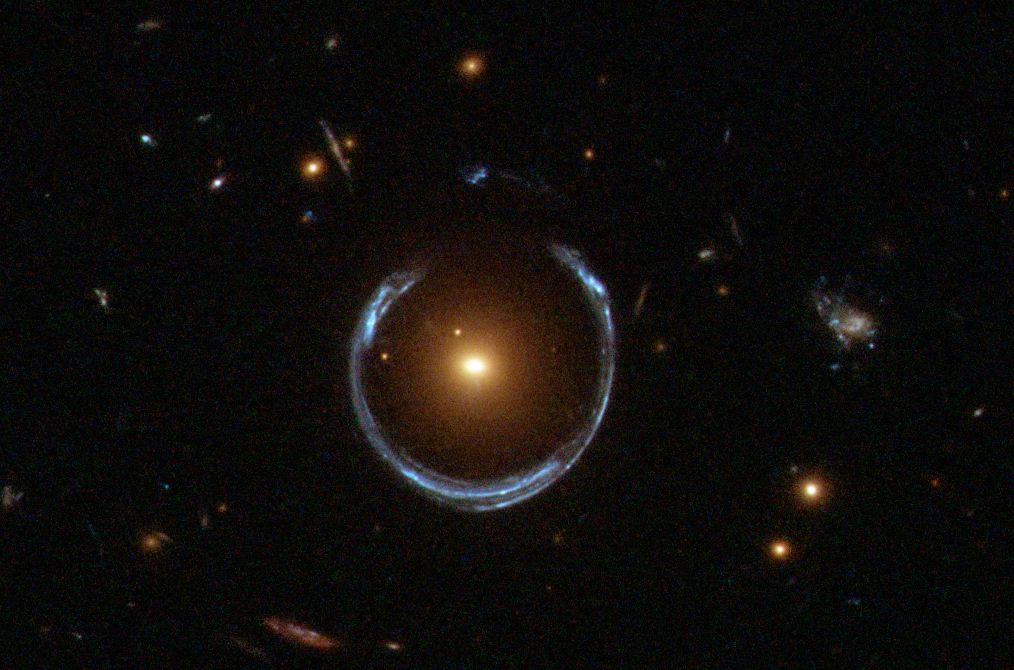
\includegraphics[width=\textwidth]{einstein_ring}
\caption{An Einstein ring}
\label{fig:einring}
\end{subfigure}
\qquad
\begin{subfigure}{0.4\textwidth}
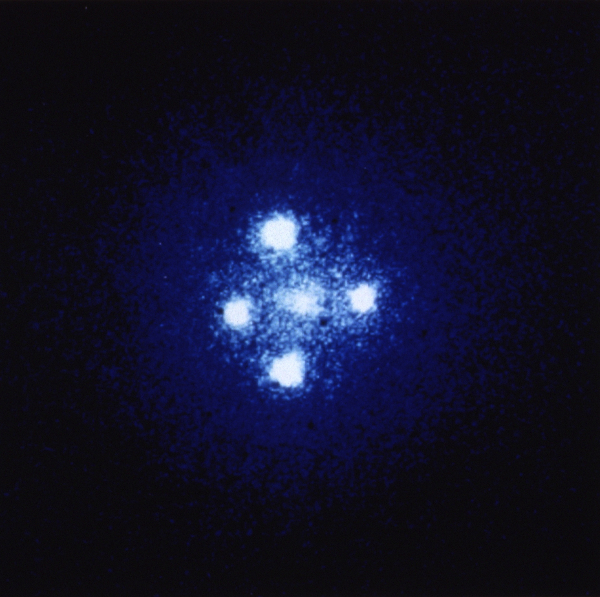
\includegraphics[width=\textwidth]{einstein_cross}
\caption{Einstein's cross}
\label{fig:einsteincross}
\end{subfigure}
\caption{Two examples of strong lensing effects. a) shows light from
a distant blue galaxy being distorted by the central galaxy LRG 3-757
\cite{einsteinring}. b) shows four images of a distant quasar being lensed by a
foreground galaxy \cite{eincross}.}
\label{fig:stronglens}
\end{figure}
\subsubsection{Importance of the Time Delay}
\label{sec-2-1-1}

In gravitationally lensed systems, there is a delay between photon streams
coming from images of the source due to the bending of light. Light from one
source may have had to travel a slightly longer distance than that from the
other, and while photons travel extremely fast, over astronomical distances the
delay can become quite large. 
\begin{itemize}
\item Talk generally about the problem of time delay estimation
\item refer to physics papers attempting to make estimates of the delay
\item talk about time delay estimation in particular, refer to kundic et al, many others
\item talk about how better estimates benefit the scientific community
\item refer to peter's paper about the efficacy of kernel regression
\item better estimators are necessary to increase the accuracy of estimates
\item this is an experiment to see whether this method has any use
\item build on technique introduced in massey et al
\end{itemize}
\subsection{Poisson Processes}
\label{sec-2-2}

In certain situations, there are many benefits of having good models of the
numbers of events that occur in a given period. For example, being able to
estimate the number of incoming requests to a server, the number of calls made
to emergency services, and the rate of radioactive decay at any given time are
all useful in different applications. Poisson processes are \emph{stochastic
processes} that can be used to do just that. A stochastic process is a way of
representing the evolution of a random value or system over time by using
collections of random variables. Most such processes do not evolve in a
\emph{deterministic} way. That is, the way they change as time passes is not
predictable.

A Poisson process is one such process which counts the number of events and the
time at which they occur in a given time interval, and have been used to model
all of the above examples
\cite{hajjam2008approach,cannizzaro1978results,arlitt1997internet}. In their
basic form, Poisson processes have the following important properties
\cite{ross1997simulation}:
\begin{enumerate}
\item $N(0)=0$.
\begin{itemize}
\item $N(t)$ represents the total number of events that occurred up until time
     $t$. Thus, if $N(0)=0$, it follows that the process begins at $t=0$.
\end{itemize}
\item The numbers of events occurring in disjoint time intervals are independent.
\begin{itemize}
\item The \emph{independent increment} assumption. This states that $N(t)$, the
     number of events that occur up to time $t$ is \emph{independent} of the
     number $N(t+s)-N(t)$, i.e. the number of events in the time interval
     between $t$ and $s$. In other words, the number of events that occur in one
     interval does not have an effect on the number of events in any other time
     interval.
\end{itemize}
\item The probability distribution of the number of events that occur in a given
   interval is dependent only on the length of the interval.
\begin{itemize}
\item The \emph{stationary increment} assumption. The implication of this is that
     the probability distribution of $N(t+s)-N(t)$ is the same for all values of
     $t$. That is, the likelihood of a number of events $n$ occurring in the
     above time interval does not change, regardless of the value of $t$.
\end{itemize}
\item No counted occurrences are simultaneous.
\begin{itemize}
\item For all events that occur in the duration of the process, no two events
     will occur at the same time.
\end{itemize}
\end{enumerate}
Note the rate parameter cannot be below zero
\begin{itemize}
\item where do they occur
\item what can they be used for
\item Times for a homogeneous poisson process can be generated using
     the formula $\log\frac{-U}{\lambda}$
\end{itemize}
\subsection{Linear Regression}
\label{sec-2-3}
\section{Simulation of Photon Streams}
\label{sec-3}
\subsection{Function Generation}
\label{sec-3-1}
\subsection{Generating Streams from Functions}
\label{sec-3-2}
\section{Function Estimation}
\label{sec-4}
\subsection{Baseline Estimation}
\label{sec-4-1}
\subsubsection{Optimum Least Squares}
\label{sec-4-1-1}
\subsubsection{Iterative Weighted Least Squares}
\label{sec-4-1-2}
\subsubsection{Piecewise Iterative Weighted Least Squares}
\label{sec-4-1-3}

    Initially, we thought that it may be possible to decide whether to
    extend the line or not based on the difference in slope between
    the estimate from the previous time interval and the estimate of
    the next. If the previous estimate was positive, and the next
    negative, and vice versa, clearly the line should not be
    continued. The intercept parameter was considered to be much less
    important. However, this assumption was highly flawed. Due to the
    nature of poisson processes, it is perfectly possible that
    although the function has changed significantly after the end of
    the previous interval, the estimate for the interval that we are
    trying to extend the line into could return very similar values to
    that of the previous interval. Because of this, we extend the line
    when we should not be doing so. There are several potential
    solutions to this problem. First, rather than forming a new
    estimate, we extend the line and then check how much the error has
    increased. If it goes over a certain threshold, then we reject the
    extension attempt and try again, this time with a shorter
    extension. Another potential way of improving the piecewise
    estimation in general would be to require the estimate for the
    next time period to start from the end point of the last time
    period. This would prevent the intercept parameter from changing,
    and would force the estimator to find the best estimate given a
    specific starting point, rather than giving it free reign to find
    the estimate which actually minimises the error.
\begin{itemize}

\item coding issues\\
\label{sec-4-1-3-1}%
what to do with the issue of minimum length of intervals? Sometimes
not extending the original gives a better estimate of the line than
re-estimating the interval extended, or adding the short interval onto
the end of the previous one and using its estimate. See data in the
min$_{\mathrm{interval}}$$_{\mathrm{length}}$ folder in data. The better fitting line is the
baseline estimate of that with no minimum, and the other set is the
estimate with minimum interval length applied
\end{itemize} % ends low level
\subsubsection{Baseline}
\label{sec-4-1-4}
\subsection{Kernel Density Estimation}
\label{sec-4-2}
\section{Time Delay Calculation}
\label{sec-5}
\subsection{Area Method}
\label{sec-5-1}
\subsection{Probability Mass Function Method}
\label{sec-5-2}
\section{System}
\label{sec-6}
\subsection{System Structure}
\label{sec-6-1}
\subsubsection{Overall Structure}
\label{sec-6-1-1}
\subsubsection{Estimators}
\label{sec-6-1-2}
\subsubsection{Generators}
\label{sec-6-1-3}
\subsubsection{Experimenter}
\label{sec-6-1-4}
\subsection{Development}
\label{sec-6-2}
\subsubsection{Development Process}
\label{sec-6-2-1}
\subsubsection{Version Control}
\label{sec-6-2-2}

\begin{itemize}
\item branching strategy
\item commit frequency
\item using issues on github
\end{itemize}
\subsubsection{Project Management}
\label{sec-6-2-3}

\begin{itemize}
\item keep changelog
\item writing up and planning layout in notebook
\end{itemize}
\section{Evaluation}
\label{sec-7}
\subsection{experimentation on simulated data}
\label{sec-7-1}
\subsection{experimentation on real-world data}
\label{sec-7-2}
\section{Conclusion}
\label{sec-8}

\newpage
\printbibliography
\newpage
\begin{appendices}
\section{Installation}
\label{sec-9}
\subsection{MuParser}
\label{sec-9-1}

 download package\\
 run \texttt{./configure --prefix=/usr}, followed by \texttt{make \&\& make install} (may require sudo)
 this installs muparser so that headers can be found in \texttt{/usr/include}
 \begin{verbatimtab}   
 sudo apt-get install libgsl0-dev check 
 \end{verbatimtab}
\section{Usage}
\label{sec-10}
\subsection{Creating functions for experimentation}
\label{sec-10-1}

   Generate 10 random functions using gaussians, and output the transforms as
   well so they can be plotted
   \begin{verbatimtab}
   ./launcher -g ../data/params.txt -r -t 2 -c 10
   \end{verbatimtab}
   Generate two streams from each of these generated functions using the
   gaussian generator
   \begin{verbatimtab}
   ./launcher -g ../data/params.txt -f rand -n 2 -c 10
   \end{verbatimtab}
   Generate stuttered streams from files in this directory, so that you can
   perform model fitting to find the best parameters to use on the generated
   set.
   \begin{verbatimtab}
   ./launcher -x ../data/exp_params.txt -p ../data/params.txt -c 10 -n 2 -s -i .
   \end{verbatimtab}
   
\end{appendices}

\end{document}